\begin{figure}[h!]
\textbf{Tema d'Esame di Gennaio 2015}\\ \\
Si determini la differenza di potenziali ai capi della resistenza $R4$ del circuito mostrato in figura. La differenza di potenziale fornita dalla batteria è di $12V$ e i valori delle resistenze sono rispettivamente $R2=15\Omega, R3=40\Omega, R4=25\Omega, R5=R6=32\Omega, R1=R7=18\Omega$
\begin{center}
		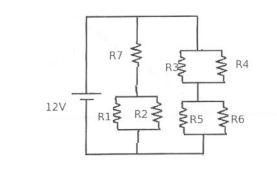
\includegraphics[scale=1.2]{ES5/GEN052015.jpg}
	\end{center}
	\begin{boxed}
		\null\hfill \textbf{Soluzione:} $V_4 = 5.85 V$\\
		\textbf{Procedimento: } \\
		Semplificazione delle Resistenze:\\
		$R_{34}=\frac{R_3\cdot R_4}{R_3+R_4}=\frac{40\Omega \cdot 25\Omega}{40\Omega+25\Omega}=15.38\Omega$\\
		$R_{56}=\frac{R_5\cdot R_6}{R_5+R_6}=\frac{32\Omega \cdot 32\Omega}{32\Omega+32\Omega}=16\Omega$\\
		$R_{12}=\frac{R_1\cdot R_2}{R_1+R_2}=\frac{18\Omega \cdot 15\Omega}{18\Omega+15\Omega}=8.18\Omega$\\
		$R_{127}=R_{12}+R_7=8.18\Omega + 18\Omega=26.18\Omega$\\
		$R_{3456}=R_{34}+R_{56}=15.38\Omega+16\Omega=31.38\Omega$\\
		$R_{tot}=\frac{R_{127}\cdot R_{3456}}{R_{127}+R_{3456}}=\frac{26.18\Omega \cdot 31.38\Omega}{26.18\Omega + 31.38\Omega}=14.23\Omega$\\
		Ricordando che la Tensione in parallelo non cambia, così come non cambia la corrente in serie:\\
		$V_{tot}=V_{127}=V_{3456}=12V$\\
		$I_{3456}=\frac{V_{3456}}{R_{3456}}=0.38A \qquad I_{3456}=I_{34}=I_{56}$\\
		$V_{34}=V_3=V_4=R_{34}\cdot I_{34}=15.38\Omega \cdot 0.38A=5.85\Omega \qquad V_{34}=V_3=V_4$
	\end{boxed}
\end{figure}

\begin{figure}[h!]
\textbf{Tema d'Esame di Febbraio 2015}\\ \\
 Nel circuito in figura, la corrente attraverso $R6$ è $i_6=1.40A$ e le resistenze sono
$R1=R2=R3=2.0\Omega, R4= 16.0\Omega, R5= 8.0 \Omega e R6= 4.0 \Omega$. Qual'è la forza elettromotrice della batteria (ideale)?
\begin{center}
		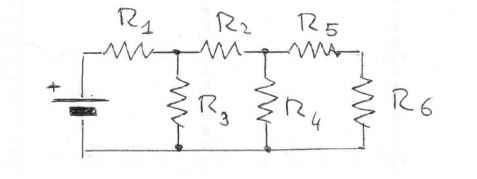
\includegraphics[scale=0.8]{ES5/FEB052015.jpg}
	\end{center}
\end{figure}

\begin{figure}[h!]
\textbf{Tema d'Esame di Giugno 2015}\\ \\
Si determini la differenza di potenziali ai capi della resistenza R4 del circuito mostrato in figura. La differenza di potenziale fornita dalla batteria è di $12V$ e i valori delle resistenze sono rispettivamente $R2=15\Omega, R3=40\Omega, R4=25\Omega, R5=R6=32\Omega, R1=R7=18\Omega$.
\begin{center}
		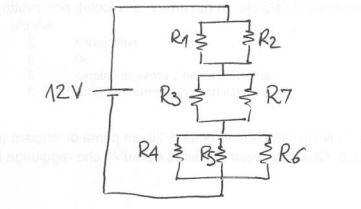
\includegraphics[scale=1]{ES5/GIU052015.jpg}
	\end{center}
\end{figure}

\begin{figure}[h!]
\textbf{Tema d'Esame di Luglio 2015}\\ \\
La differenza di potenziale fornita dalla batteria è di $12V$ e i valori delle resistenze sono rispettivamente $R2=15\Omega, R3=40\Omega, R4=25\Omega, R5=R6=32\Omega, R1=R7=18\Omega$
\begin{center}
		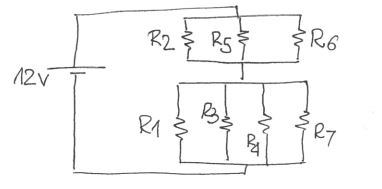
\includegraphics[scale=1]{ES5/LUG052015.jpg}
	\end{center}
\end{figure}